\documentclass[border=10pt]{standalone}

\usepackage{tikz}
\usepackage{tikzsymbols}
\usetikzlibrary{calc,patterns,shapes.geometric}

\def\centerarc[#1](#2)(#3:#4:#5){\draw[#1] ($(#2)+({#5*cos(#3)},{#5*sin(#3)})$) arc (#3:#4:#5);}

\begin{document}
	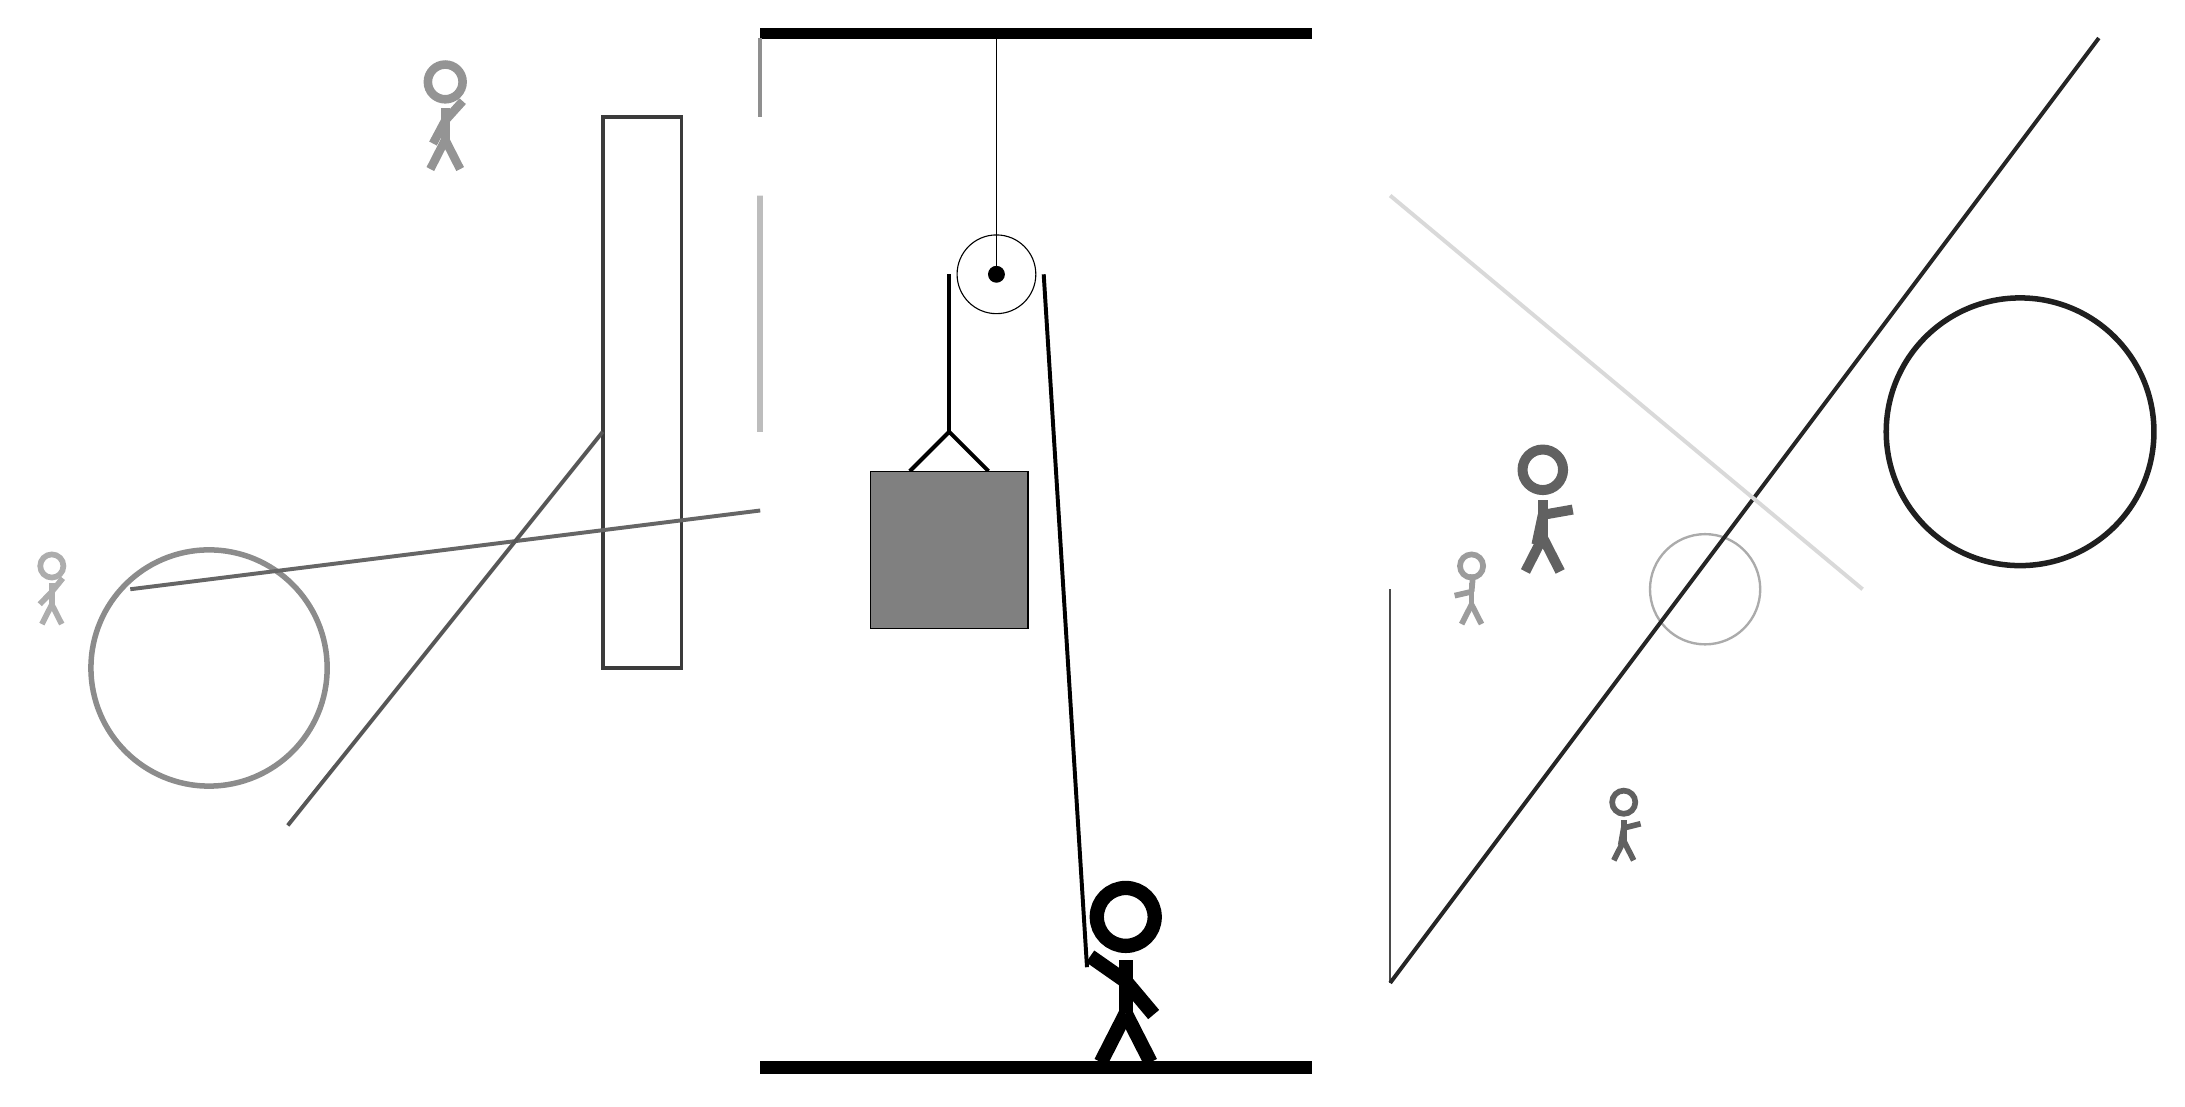
\begin{tikzpicture}
		%%%%% START %%%%%
		
		\draw[fill=black] (-2, 10) rectangle (5, 10.125);
		
		\node[line width=0.7mm, color=black!62] at (9, 0) {\Strichmaxerl[4][80][14]};
		
		\draw [line width=0.7mm, color=black!45](-9, 2) circle (1.5);
		\draw[line width=0.7mm, color=black!26] (-2, 5) rectangle (-2, 8);
		\node[line width=0.3mm, color=black!39] at (7, 3) {\Strichmaxerl[4][13][85]};
		\draw[line width=0.5mm, color=black!77] (-3, 2) rectangle (-4, 9);
		\draw[line width=0.2mm, color=black!71] (6, 3) rectangle (6, -2);
		\draw[line width=0.5mm, color=black!44](-2, 9) -- (-2, 10);
		
		\draw[line width=0.5mm, color=black!60](-2, 4) -- (-10, 3);
		\node[line width=0.2mm, color=black!62] at (8, 4) {\Strichmaxerl[7][78][10]};
		
		\node[line width=0.4mm, color=black!32] at (-11, 3) {\Strichmaxerl[4][46][51]};
		\draw [line width=0.7mm, color=black!88](14, 5) circle (1.7);
		\draw [line width=0.3mm, color=black!33](10, 3) circle (0.7);
		\draw[line width=0.5mm, color=black!85](6, -2) -- (15, 10);
		\node[line width=0.6mm, color=black!42] at (-6, 9) {\Strichmaxerl[6][62][48]};
		\draw[line width=0.5mm, color=black!15](6, 8) -- (12, 3);
		\draw[line width=0.5mm, color=black!66](-4, 5) -- (-8, 0);
		
		
		\draw (1, 7) circle (0.5);
		\draw[fill=black] (1, 7) circle (0.1);
		\draw (1, 10) -- (1, 7);
		
		\draw[line width=0.5mm] (-0.1, 4.5) -- (0.4, 5.0) -- (0.9, 4.5);
		\draw[fill=black!50] (-0.6, 4.5) rectangle (1.4, 2.5);
		
		\draw[line width=0.5mm] (0.4, 7) -- (0.4, 5.0);
		\centerarc[line width=0.5mm](1, 7)(0:180:0.6);
		\draw[line width=0.5mm](1.6, 7) -- (2.15, -1.8);
		
		\node at (2.6, -1.9) {\Strichmaxerl[10][-35][-50]};
		
		\draw[fill=black] (-2, -3) rectangle (5, -3.15);
		
		%%%%% END %%%%%
	\end{tikzpicture}
\end{document}